\documentclass[11pt,a4paper]{article}

\usepackage[T1]{fontenc}
\usepackage{lmodern}
\usepackage{microtype}
\emergencystretch=2em
\usepackage{geometry}
\geometry{a4paper,top=24mm,bottom=24mm,left=25mm,right=25mm,headheight=14pt,footskip=12mm}
\usepackage{amsmath,amssymb,bm}
\usepackage[table]{xcolor}
\definecolor{primary}{RGB}{0,51,102}
\definecolor{secondary}{RGB}{41,128,185}
\definecolor{headerbg}{gray}{0.92}
\usepackage{titlesec}
\titleformat{\section}{\normalfont\Large\bfseries\color{primary}}{\thesection}{1em}{}[\color{secondary}\titlerule]
\titleformat{\subsection}{\normalfont\large\bfseries\color{secondary}}{\thesubsection}{1em}{}
\usepackage{fancyhdr}
\pagestyle{fancy}
\fancyhf{}
\fancyhead[L]{\small\color{gray}RAG-informed 2.4 GHz RNI sensor}
\fancyhead[R]{\small\color{gray}\nouppercase{\leftmark}}
\fancyfoot[C]{\small\thepage}
\usepackage{booktabs,longtable,array,tabularx,enumitem}
\setlist{nosep,leftmargin=1.5em}
\newcolumntype{L}[1]{>{\raggedright\arraybackslash}p{#1}}
\newcolumntype{C}[1]{>{\centering\arraybackslash}p{#1}}
\newcolumntype{R}[1]{>{\raggedleft\arraybackslash}p{#1}}
\usepackage{graphicx}
\usepackage{tikz}
\usetikzlibrary{arrows.meta,positioning,shapes.geometric}
\usepackage{hyperref}
\hypersetup{colorlinks=true,linkcolor=primary,citecolor=secondary,urlcolor=secondary,
  pdfauthor={Universidad Nacional de Colombia},
  pdftitle={RAG-informed Design of an Indoor 2.4 GHz RNI Early-warning Sensor},
  pdfsubject={Triaxial antenna array, SP4T RF switching, SDR measurement, exposure assessment}}
\bibliographystyle{IEEEtran}

\title{\textbf{\LARGE\color{primary} RAG-informed Design of an Indoor 2.4 GHz RNI Sensor}\\[0.4em]
\large\color{secondary} Triaxial Antenna Array, SP4T RF Switching, Calibration, Measurement Math, and Normative Scope}
\author{Research \& Development Group\\Universidad Nacional de Colombia}
\date{\today}

\begin{document}
\maketitle
\thispagestyle{plain}

\begin{abstract}
This report specifies a low-cost, software-defined radio (SDR) prototype for monitoring radiofrequency non-ionizing radiation (RNI) in indoor environments in the 2.4 GHz ISM band. Three antenna paths are selected sequentially by an SP4T switch; the fourth switch terminal is reserved for a 50~ohm terminator or reference path. A band-pass filter limits the monitored RF path before a PlutoSky R2 receiver. The design reconstructs a calibrated total field estimate from sequential samples and produces configurable early warnings. The instrument is not presented as a legally certified compliance meter. Normative recommendations, exposure reference levels, equipment requirements, calibration, uncertainty, and limitations are separated from component datasheet facts.
\end{abstract}

\tableofcontents
\newpage

\section{Purpose and Design Boundary}

\subsection{Purpose}
The purpose of the system is to provide an indoor screening and early-warning device for elevated RF exposure in the 2.4~GHz ISM band. The intended users receive a calibrated trend, a field-strength estimate where the field model is valid, and an alert when a configurable threshold is exceeded. The device is intended to support investigation and operational awareness, not to replace a laboratory or regulatory assessment.

ITU-T K.91 covers assessment and monitoring of RF electromagnetic fields in areas with wireless devices and telecommunication installations \cite{ITU-T-K.91}. ITU-T K.61 states that calibrated instruments and correctly expressed uncertainty are required when measurements are used for compliance assessment \cite{ITU-T-K.61}. This prototype therefore reports its measurement quality and limitations instead of claiming compliance from an unverified reading.

\subsection{Normative and regulatory boundary}
The design uses the following hierarchy:
\begin{enumerate}
  \item ICNIRP 2020 supplies the exposure reference levels for 100~kHz--300~GHz \cite{ICNIRP-2020}.
  \item ITU-T K.52, K.61, K.91, K.100, and K.113 provide exposure-assessment and measurement guidance \cite{ITU-T-K.52,ITU-T-K.61,ITU-T-K.91,ITU-T-K.100,ITU-T-K.113}.
  \item IEC 62232 and IEC 62311 provide referenced measurement and equipment frameworks \cite{IEC-62232,IEC-62311}.
  \item Decreto 1370 de 2018 and ANE Resolution 0773 of 2023 define Colombian regulatory responsibilities and conditions for applicable radioelectric stations \cite{Decreto-1370-2018,ANE-0773-2023}.
\end{enumerate}

The last category does not automatically make an indoor 2.4~GHz prototype a DCER instrument. A formal Colombian compliance result requires the applicable station, procedure, calibration traceability, uncertainty statement, and regulatory documentation.

\subsection{Claims made by this report}
\begin{table}[ht]
\centering
\caption{Claim boundary for the prototype.}
\begin{tabularx}{\textwidth}{L{0.30\textwidth}X}
\toprule
\textbf{Claim} & \textbf{Position}\\
\midrule
2.4~GHz RF screening & Supported after frequency-response and field calibration.\\
Total-field estimate & Supported only after validating the antenna-array response matrix and sequential-axis stability.\\
Exposure early warning & Supported as a configurable engineering alert with a documented averaging basis.\\
Legal compliance certification & Out of scope. Requires an applicable validated procedure and laboratory-quality traceability.\\
\bottomrule
\end{tabularx}
\end{table}

\section{System Architecture and BOM Context}

\subsection{Signal path}
The RF path required by the project BOM is:
\begin{center}
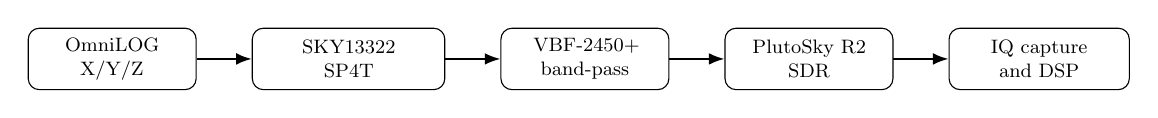
\begin{tikzpicture}[scale=0.78,transform shape,node distance=7mm and 9mm, every node/.style={font=\small},
  block/.style={draw, rounded corners, align=center, minimum height=10mm, text width=25mm},
  line/.style={-{Latex[length=2mm]}, thick}]
  \node[block] (ant) {OmniLOG\\X/Y/Z};
  \node[block,right=of ant,text width=29mm] (sw) {SKY13322\\SP4T};
  \node[block,right=of sw] (filter) {VBF-2450+\\band-pass};
  \node[block,right=of filter] (sdr) {PlutoSky R2\\SDR};
  \node[block,right=of sdr,text width=27mm] (dsp) {IQ capture\\and DSP};
  \draw[line] (ant)--(sw);
  \draw[line] (sw)--(filter);
  \draw[line] (filter)--(sdr);
  \draw[line] (sdr)--(dsp);
\end{tikzpicture}
\end{center}

The first three SP4T throws connect to the three antenna outputs. The fourth throw is not an unused open circuit: it is connected to a known 50~ohm terminator, or to a characterized reference path when the calibration procedure requires it. The selected state must be logged with every measurement block.

\subsection{Component facts from the RAG datasheets}
\begin{longtable}{L{0.23\textwidth}L{0.27\textwidth}L{0.42\textwidth}}
\caption{BOM facts and design implications.}\\
\toprule
\textbf{Part} & \textbf{RAG datasheet fact} & \textbf{Design implication}\\
\midrule
\endfirsthead
\toprule
\textbf{Part} & \textbf{RAG datasheet fact} & \textbf{Design implication}\\
\midrule
\endhead
OmniLOG 90200 & 700~MHz--2.5~GHz, 50~ohm, typical VSWR below 3:1 \cite{OmniLOG-90200} & 2.4~GHz is close to the upper frequency limit. Use the vendor antenna factor or a controlled-field calibration; do not infer a precise AF from the gain plot alone.\\
SKY13322-375LF-EVB & SP4T, 20~MHz--6~GHz; 0.60--0.75~dB typical insertion loss from 1--2.5~GHz; 26~dB typical isolation in that range; 60~ns RF switching \cite{SKY13322-375LF-EVB} & Use three throws for X/Y/Z and the fourth for a 50~ohm termination/reference. Include measured port loss and isolation in calibration.\\
VBF-2450+ & 2400--2550~MHz passband, 2450~MHz center, maximum 4~dB passband insertion loss, typical 14~dB return loss \cite{VBF-2450} & Rejects out-of-band energy but aggregates all energy in its passband. It does not identify individual Wi-Fi, Bluetooth, or Zigbee sources.\\
PlutoSky R2 & AD9361 variant: 70~MHz--6~GHz and up to 56~MHz bandwidth; AD9363 variant: up to 20~MHz bandwidth \cite{PlutoSky-R2} & Select the exact SKU. The full 2.4~GHz ISM band cannot be captured in one instantaneous recording; use segmented sweeps or declare a narrower monitored band.\\
\bottomrule
\end{longtable}

\subsection{BOM prices and procurement links}
Table~\ref{tab:bom-prices} reproduces the project BOM prices in USD. Prices are planning values from \texttt{context/BOM.md}, not quotations or a complete cost of compliance calibration. The three OmniLOG units provide the X, Y, and Z antenna paths. The SMA terminator is assigned to the fourth SP4T throw; it is not an additional antenna.

\begin{table}[ht]
\centering
\small
\caption{Project BOM prices and procurement links.}\label{tab:bom-prices}
\begin{tabularx}{\textwidth}{L{0.29\textwidth}C{0.07\textwidth}R{0.12\textwidth}R{0.13\textwidth}X}
\toprule
\textbf{Part} & \textbf{Qty.} & \textbf{Unit (USD)} & \textbf{Total (USD)} & \textbf{Supplier link}\\
\midrule
VBF-2450+ & 1 & 57.50 & 57.50 & \href{https://www.digikey.com/en/products/detail/mini-circuits/VBF-2450/27669500}{Digi-Key}\\
SKY13322-375LF-EVB & 1 & 108.93 & 108.93 & \href{https://www.digikey.com/en/products/detail/skyworks-solutions-inc/SKY13322-375LF-EVB/2356519}{Digi-Key}\\
Hosyond LCD Display & 1 & 45.99 & 45.99 & \href{https://www.amazon.com/-/es/Hosyond-pantalla-pulgadas-capacitiva-Raspberry/dp/B09XKC53NH/}{Amazon}\\
PlutoSky R2 7020 & 1 & 175.00 & 175.00 & \href{https://opensourcesdrlab.com/products/plutosky-r2?VariantsId=10403}{OpenSourceSDRLab}\\
UPS HAT & 1 & 43.19 & 43.19 & \href{https://www.amazon.com/Uninterruptible-UPS-HAT-Raspberry-Bi-Directional/dp/B0DLW2G9K6}{Amazon}\\
Samsung 21700 battery & 4 & 15.00 & 60.00 & \href{https://www.mercadolibre.com.co/1-x-bateria-de-litio-samsung-21700-recargable-5000mah-37v/p/MCO2084532948}{MercadoLibre}\\
OmniLOG 90200 & 3 & 115.76 & 347.28 & \href{https://aaronia.com/es/breitband-antenne-omnilog-90200}{Aaronia}\\
2467938-1 SMA terminator & 1 & 2.78 & 2.78 & \href{https://www.digikey.com/en/products/detail/te-connectivity-linx/2467938-1/22535225}{Digi-Key}\\
\midrule
\textbf{Total} & & & \textbf{840.67} & \\
\bottomrule
\end{tabularx}
\end{table}

The RF path is therefore three OmniLOG antenna outputs plus the 50~ohm terminator into the SP4T, followed by the VBF-2450+ and PlutoSky R2. The display, UPS, and batteries support the portable enclosure but are not part of the calibrated RF transfer function.

\subsection{SP4T acquisition model}
The SP4T solution is explicitly allowed by the measurement guidance when a single-axis antenna is positioned in orthogonal directions and the results are post-processed to obtain total field strength \cite[Sec.~9.2 and Table~I.1 footnote~b]{ITU-T-K.100}. K.113 says that three-axis readings should \emph{preferably} be simultaneous, which is a quality recommendation rather than a prohibition on a sequential implementation \cite[Sec.~7.1.1]{ITU-T-K.113}.

The sequential implementation is valid only when the temporal behavior is characterized. For each cycle, the firmware shall:
\begin{enumerate}
  \item select X, wait for the measured settling interval, and acquire a block;
  \item select Y, repeat the process, and retain timestamps;
  \item select Z, repeat the process;
  \item optionally select the fourth terminated port for a noise/reference check;
  \item reject the cycle if the field changes beyond the configured stationarity tolerance.
\end{enumerate}

This design is suitable for stable or slowly varying fields. It is not suitable for reconstructing a fast transient as if all three components had been sampled at one instant.

\section{Frequency Plan and Exposure Quantity}

\subsection{2.4 GHz band coverage}
The VBF-2450+ is wider than the nominal 2.4~GHz ISM allocation and the PlutoSky instantaneous bandwidth is narrower than that allocation. The system shall therefore store:
\begin{itemize}
  \item the center frequency and sample bandwidth of every capture;
  \item the frequency response correction applied to that segment;
  \item the segments that were measured and any frequency gaps;
  \item whether the result is a band aggregate or a frequency-selective estimate.
\end{itemize}

Frequency-selective measurements are preferred when individual sources or frequency-dependent limits must be distinguished; broadband measurements provide the aggregate within the instrument bandwidth \cite[Sec.~9.2]{ITU-T-K.100}. The early-warning display can use the aggregate 2.4~GHz band result. Raw spectral segments remain available for diagnosis.

\subsection{Applicable ICNIRP quantities at 2.4 GHz}
At frequencies above 2~GHz, ICNIRP 2020 gives power-density reference levels rather than an E-field reference level in the summarized tables \cite[Tables~5--6]{ICNIRP-2020}. For general public exposure, the values relevant to this design are:
\begin{itemize}
  \item whole-body average over 30 minutes: $S_{\mathrm{RL}}=10\ \mathrm{W/m^2}$;
  \item local exposure average over 6 minutes: $S_{\mathrm{RL}}=40\ \mathrm{W/m^2}$.
\end{itemize}

In a far-field plane-wave region, the engineering conversion is:
\begin{equation}
  S \simeq \frac{E_{\mathrm{rms}}^2}{\eta_0},
  \qquad \eta_0 \simeq 377\ \Omega .
  \label{eq:plane-wave}
\end{equation}
Thus, equivalent screening values are approximately 61.4~V/m for 10~W/m$^2$ and 122.8~V/m for 40~W/m$^2$. These are derived E-field values, not independent ICNIRP E-field reference levels. In the reactive near field, E and H are not proportionally related; K.91 requires both field components or assessment of the applicable basic restrictions \cite[Sec.~7.2.6]{ITU-T-K.91}.

\section{Calibrated Measurement Model}

\subsection{Antenna factor}
For each axis and frequency, the antenna factor is:
\begin{equation}
  AF_k(f)=\frac{E_{\mathrm{ref}}(f)}{V_{\mathrm{in},k}(f)}\quad [\mathrm{m^{-1}}],
  \label{eq:af}
\end{equation}
where $V_{\mathrm{in},k}$ is the calibrated voltage at the antenna/receiver reference plane. This is the definition given by K.61 \cite[Sec.~8.1.3.2]{ITU-T-K.61}; the AF shall be known with its uncertainty. For broadband probes with internal processing, K.61 distinguishes the calibration factor $CF=E_{\mathrm{ref}}/E_{\mathrm{meas}}$ from the raw antenna factor \cite[Sec.~8.1.3.1]{ITU-T-K.61}.

\subsection{Receiver and switch calibration}
Let $d_k[n]$ be the corrected digital IQ sample for axis $k$, after DC-offset removal and any validated IQ correction. Define:
\begin{equation}
  D_{k,\mathrm{rms}}=
  \sqrt{\frac{1}{M_k}\sum_{n=1}^{M_k}
  \left(d_{I,k}^2[n]+d_{Q,k}^2[n]\right)}.
  \label{eq:digital-rms}
\end{equation}
Rather than assuming a generic ADC full-scale voltage, determine a calibrated factor $C_k(f)$ in volts per digital unit:
\begin{equation}
  V_{\mathrm{in},k}(f)=C_k(f)D_{k,\mathrm{rms}}.
  \label{eq:receiver-cal}
\end{equation}
$C_k(f)$ includes receiver gain, cable loss, filter loss, switch insertion loss, connector loss, and the chosen digital scaling. If the same receiver is shared, most terms are common, but switch-port and antenna-path differences remain axis-specific.

\subsection{Field reconstruction}
The ideal diagonal-axis model is:
\begin{equation}
  E_{k,\mathrm{rms}}(f)=AF_k(f)C_k(f)D_{k,\mathrm{rms}}.
  \label{eq:axis-field}
\end{equation}
If the three antenna outputs are demonstrated to be orthogonal field components, the total field is:
\begin{equation}
  E_{\mathrm{total,rms}}(f)=
  \sqrt{E_x^2(f)+E_y^2(f)+E_z^2(f)}.
  \label{eq:rss}
\end{equation}
K.100 §9.2 permits single-axis antennas when the individual contributions are post-processed in this way; K.91 Equation 7-5 gives the corresponding RSS treatment for RMS values \cite{ITU-T-K.100,ITU-T-K.91}.

\subsection{Transfer-matrix correction}
The OmniLOG 90200 datasheet describes a broadband omnidirectional antenna, not a calibrated ideal dipole component. Therefore the design shall not assume that three mechanically orthogonal antennas automatically measure ideal Cartesian components. During calibration, use a known field with multiple orientations to estimate:
\begin{equation}
  \bm{e}(f)=\bm{T}(f)\bm{d}(f),
  \qquad
  E_{\mathrm{total}}(f)=\|\bm{e}(f)\|_2,
  \label{eq:matrix}
\end{equation}
where $\bm{d}$ contains the three calibrated axis outputs and $\bm{T}$ is the measured complex or real response matrix. The diagonal AF/RSS model in Equation~\ref{eq:rss} is a special case of Equation~\ref{eq:matrix}. The matrix must be used if cross-axis coupling, polarization response, or non-orthogonal sensitivity is material.

\section{Sequential RMS and Early-Warning Algorithm}

\subsection{Acquisition timing}
The switch datasheet reports 60~ns RF switching characteristics \cite{SKY13322-375LF-EVB}; this is not the complete system settling time. The implemented settling interval shall be measured with the actual control electronics, SDR configuration, filter, and signal. The first samples after every transition are discarded:
\begin{equation}
  M_{\mathrm{discard},k}=\left\lceil t_{\mathrm{settle},k}f_s\right\rceil .
  \label{eq:discard}
\end{equation}

\subsection{Time averaging}
ICNIRP 2020 specifies 6-minute averaging for local exposure and 30-minute averaging for whole-body exposure in the relevant 2.4~GHz reference-level framework \cite[Tables~5--6]{ICNIRP-2020}. K.91 explains that averaging time is based on tissue thermal time constants, not merely on communication-signal variation \cite[Sec.~7.2.3]{ITU-T-K.91}.

The firmware should maintain rolling sums of calibrated power or squared field values rather than storing all raw samples for 6 or 30 minutes. A sequential X/Y/Z cycle may be used for screening, but it shall carry a temporal-quality flag because its components do not correspond to the same instant. A full exposure assessment should use a validated cycle duration and, where required, a separate simultaneous or conservative measurement procedure.

\subsection{Alert calculation}
For far-field screening at 2.4~GHz, calculate:
\begin{equation}
  S_{\mathrm{est}}=\frac{E_{\mathrm{total,rms}}^2}{377},
  \qquad
  ER=\frac{S_{\mathrm{est}}}{S_{\mathrm{RL}}}.
  \label{eq:alert}
\end{equation}
The application may define advisory and warning thresholds as fractions of the selected reference level. The displayed result shall include the threshold basis, averaging interval, frequency coverage, and quality state. It shall not display ``compliant'' solely because $ER<1$.

For multiple frequency segments, the exposure ratio must use the applicable frequency-specific limits and combine contributions consistently. K.91 Equation 7-5 and K.100 §9.7 provide the basis for RSS/total-exposure post-processing \cite{ITU-T-K.91,ITU-T-K.100}. The filter-only aggregate cannot support source-specific TER without frequency-selective segmentation.

\section{Calibration and Verification Plan}

\subsection{Required calibration stages}
\begin{enumerate}
  \item \textbf{Antenna calibration:} obtain the vendor AF/certificate for each OmniLOG unit, or calibrate the assembled array in a known field. K.61 requires AF as a frequency function and specifies its uncertainty expectation \cite[Sec.~8.1.3.2]{ITU-T-K.61}.
  \item \textbf{RF-path calibration:} measure each SP4T port, the VBF-2450+ insertion loss, cables, connectors, and SDR response at the antenna reference plane.
  \item \textbf{Array calibration:} estimate $\bm{T}(f)$ using known polarization and orientation conditions. Verify cross-axis coupling, isotropy, and repeatability. K.61 identifies isotropy error and axial rejection as relevant to a three-axis RMS result \cite[Secs.~8.1.3.3 and 8.1.3.7]{ITU-T-K.61}.
  \item \textbf{RMS validation:} apply two known RF sources separately and together. K.61 §8.1.3.6 requires verification that the result follows the RMS combination law \cite[Sec.~8.1.3.6]{ITU-T-K.61}.
  \item \textbf{Signal validation:} compare CW, modulated, and pulsed test signals when those signal classes are in scope. K.61 requires checking whether pulsed signals change the calibrated response \cite[Sec.~8.1.3.5]{ITU-T-K.61}.
  \item \textbf{Environmental validation:} test indoors with representative reflections and document the effect of the operator, enclosure, nearby objects, and antenna support.
\end{enumerate}

\subsection{Performance checks}
K.100 Appendix I and Table I.1 provide equipment-oriented requirements, including frequency response, dynamic range, linearity, signal-to-noise ratio, and isotropy expectations \cite[Appendix~I]{ITU-T-K.100}. The prototype verification record shall report measured values against the following requirements or clearly mark them as unverified:
\begin{table}[ht]
\centering
\caption{Verification matrix.}
\begin{tabularx}{\textwidth}{L{0.32\textwidth}L{0.28\textwidth}X}
\toprule
\textbf{Check} & \textbf{Acceptance basis} & \textbf{Evidence}\\
\midrule
Frequency response & K.100 Table I.1; declared project band & Swept source and calibrated correction table.\\
Linearity & K.100 Table I.1 and K.61 §8.1.3.4 & Multiple input levels, maximum deviation reported.\\
Axis response & K.61 §§8.1.3.3, 8.1.3.7 & Orientation sweep, isotropy and axial rejection results.\\
Switching & SKY13322 datasheet plus measured system settling & Port loss, isolation, transition waveform, discarded samples.\\
RMS integration & K.61 §8.1.3.6 & Two-source combination test.\\
Uncertainty & K.61 §8.2; K.100 §10 & Type A/B budget and coverage factor.\\
\bottomrule
\end{tabularx}
\end{table}

\section{Uncertainty, Indoor Effects, and Limitations}

\subsection{Uncertainty budget}
Relevant contributors include antenna factor, switch/filter/cable calibration, SDR response, frequency interpolation, mismatch, isotropy, cross-axis coupling, temporal multiplexing, reflections, and operator/body scattering. K.100 Tables 10-1 and 10-2 provide example influence quantities; K.61 gives a target expanded uncertainty of no more than 4~dB for in-situ field measurements and no more than 6~dB for the exposure evaluation \cite[Sec.~8.2]{ITU-T-K.61}.

The project shall not insert invented ``typical dB'' values into the final budget. Each value must come from a measurement, certificate, datasheet tolerance, or justified distribution. For independent contributions:
\begin{equation}
  u_c=\sqrt{\sum_i(c_i u_i)^2},
  \qquad U=k u_c,
  \label{eq:uncertainty}
\end{equation}
where $u_i$ is a standard uncertainty, $c_i$ a sensitivity coefficient, and $k$ the selected coverage factor. Correlation between common receiver terms and axis terms must be considered rather than blindly combining all values in quadrature.

\subsection{Indoor field limitations}
Indoor walls, furniture, equipment, and the operator can reflect or scatter the field. The reported value is location-dependent. K.100 recommends keeping measurement equipment at least 1~m from reflecting objects and evaluating specified heights in its base-station procedure \cite[Sec.~9.4]{ITU-T-K.100}. Those procedures are useful design guidance but are not automatically the legal procedure for every indoor ISM source.

If the sensor is close to a transmitting device or antenna, the field may be in the reactive near field. In that condition, the E-only power-density conversion in Equation~\ref{eq:plane-wave} is not a compliance method. A future version should add a calibrated H-field channel or a source-specific near-field model.

\subsection{Known limitations}
\begin{itemize}
  \item Three OmniLOG units are not automatically a mathematical triaxial electric-field probe; the transfer matrix must be measured.
  \item Sequential switching introduces temporal mismatch between axes.
  \item The VBF-2450+ passband is an aggregate measurement window, not an emitter classifier.
  \item The PlutoSky variant must be fixed before defining frequency coverage and sample-rate limits.
  \item E-field-only exposure conversion is restricted to a valid plane-wave region.
  \item The prototype cannot issue a DCER or other legal compliance declaration by itself.
\end{itemize}

\section{Traceability Summary}
\begin{longtable}{L{0.25\textwidth}L{0.30\textwidth}L{0.34\textwidth}}
\caption{Requirement traceability.}\\
\toprule
\textbf{Design item} & \textbf{Source} & \textbf{Implementation response}\\
\midrule
\endfirsthead
\toprule
\textbf{Design item} & \textbf{Source} & \textbf{Implementation response}\\
\midrule
\endhead
Single-axis sequential post-processing & ITU-T K.100 §9.2 and Table I.1 footnote b & SP4T cycles X/Y/Z and computes calibrated RSS/matrix total.\\
Preferred simultaneous readings & ITU-T K.113 §7.1.1 & Timestamp axes, calculate temporal quality, reject unstable cycles.\\
Antenna factor & ITU-T K.61 §8.1.3.2 & Store AF per antenna and frequency with uncertainty.\\
Isotropy and axial rejection & ITU-T K.61 §§8.1.3.3, 8.1.3.7 & Measure array response; do not assume orthogonality.\\
RMS and multiple-signal integration & ITU-T K.61 §8.1.3.6 & Perform two-source validation.\\
2.4~GHz reference levels & ICNIRP 2020 Tables 5--6 & Use power density and declare 6/30-minute basis.\\
Colombian framework & Decreto 1370 (2018), ANE Resolution 0773 (2023) & Label prototype as screening; map formal compliance separately.\\
RF hardware & OmniLOG, SKY13322, VBF-2450+, PlutoSky datasheets & Include measured losses, exact SKU, band gaps, and fourth-port termination.\\
\bottomrule
\end{longtable}

\section{Conclusion}
The selected hardware can implement a useful indoor 2.4~GHz RNI early-warning sensor with one SDR and an SP4T switch. The fourth SP4T terminal shall be populated by a known 50~ohm terminator or characterized reference path. The central engineering requirement is not merely switching three antennas; it is validating the assembled antenna-array response, the sequential timing error, and the complete RF-to-IQ calibration. Once those measurements exist, the system can provide defensible screening values and quality-aware alerts. It must continue to distinguish those alerts from a formal exposure-compliance determination.

\newpage
\nocite{IEEE-149,ISO-IEC-17025}
\bibliography{references}

\end{document}
